\begin{tikzpicture}[->,>=stealth',shorten >=1pt, auto, thick, every text node part/.style={align=center}]
	\only<1-2>
	{
		\node[inner sep=0pt, label=above:$s_1$] (i) {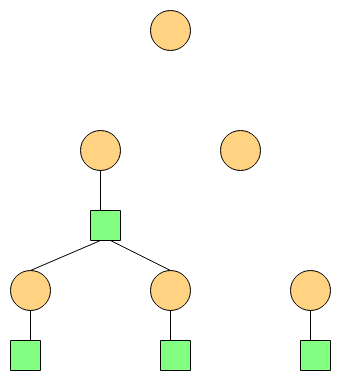
\includegraphics[scale=0.2]{../img/trajectory_i.png}};
		\node[inner sep=0pt, right=of i, label=above:$s_2$] (k1) {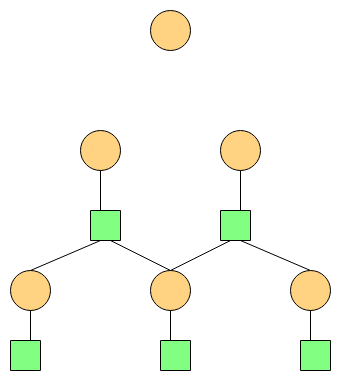
\includegraphics[scale=0.2]{../img/trajectory_k1.png}};
		\node[draw=none, right=of k1](E1){$\ldots$};
		\node[inner sep=0pt, right=of E1, label=above:$s_T$] (k2) {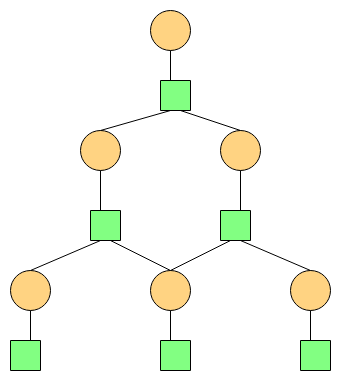
\includegraphics[scale=0.2]{../img/trajectory_k2.png}};
    \node[draw=none, right=0pt of k2](R1){$\vec{r}_1[a_1]$};
		
		\path[->]
		  (i) edge node[above]{$a_1$} (k1)
  		(k1) edge node[above]{$a_2$} (E1)
  		(E1) edge node[above]{$a_{T-1}$} (k2);
	}
	\visible<2>
	{
		\node[inner sep=0pt, below=of k1, label=above:$s_2'$] (p1) {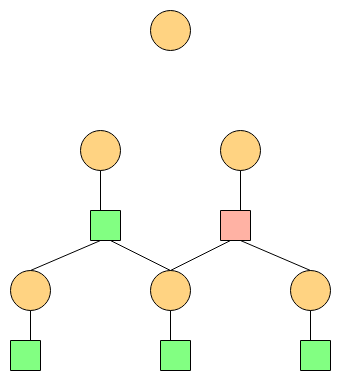
\includegraphics[scale=0.2]{../img/trajectory_p1.png}};
		\node[draw=none, right=of p1](E2){$\ldots$};
		\node[inner sep=0pt, right=of E2, label=above:$s_T'$] (p2) {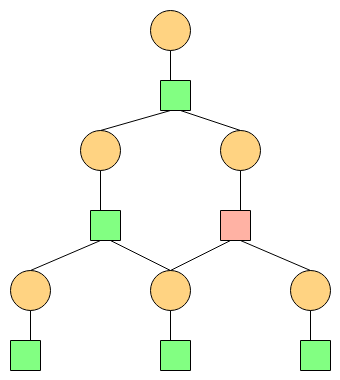
\includegraphics[scale=0.2]{../img/trajectory_p2.png}};
    \node[draw=none, right=0pt of p2](R2){$\vec{r}_1[a_1']$};
		
		\path[->]
  		(p1) edge node[above]{$a_2'$} (E2)
  		(E2) edge node[above]{$a_{T-1}'$} (p2)
  		(i) edge[bend right] node[above]{$a_1'$}(p1); 
	}
\end{tikzpicture} 
